\documentclass[../../norme-di-progetto.tex]{subfiles}

\begin{document}

\subsubsection{Finalità}%
\label{subs:sviluppo/finalita}

GruppOne istanzia il processo di sviluppo per realizzare il prodotto richiesto dal proponente.

\subsubsection{Descrizione}%
\label{subs:sviluppo/descrizione}

Il processo di sviluppo fissa quali sono gli obiettivi dello sviluppo, dalla creazione alla consegna del prodotto finale.

Raggruppa le seguenti attività:
\begin{itemize}
  \item Analisi dei requisiti
  \item Progettazione
  \item Codifica
  \item Testing
  \item Installazione.
\end{itemize}

\subsubsection{Attività}%
\label{subs:sviluppo/attivita}

\paragraph{Analisi dei requisiti}%
\label{par:analisi_dei_requisiti}
L'analisi dei requisiti è l'attività che studia e comprende il dominio applicativo del problema e ha come scopo quello di offrire i requisiti che dovranno essere soddisfatti dal software.

Si articola nei seguenti compiti:

\begin{itemize}
  \item Delineare i casi d'uso del sistema a partire dal capitolato e dallo \textit{studio di fattibilità}.
  \item Realizzare i diagrammi UML dei casi d'uso.
  \item Determinare i requisiti impliciti ed espliciti del sistema.
  \item Classificare i requisiti.
  \item Ricavare i requisiti atomici da fornire ai progettisti perché possano iniziare l'attività di progettazione.
\end{itemize}

Il documento di riferimento, \textit{Analisi dei requisiti}, è redatto dagli analisti.

\subparagraph{Classificazione dei requisiti}%
\label{subp:classificazione_dei_requisiti}

Per identificare i requisiti in maniera univoca, GruppOne ha deciso di adottare delle norme per la classificazione dei requisiti.
Ogni requisito è caratterizzato da un codice alfanumerico così formato:
\begin{center}
  \textbf{R[numero][tipo][priorità]}
\end{center}
in cui ogni elemento ha un diverso significato:
\begin{description}
  \item [numero] indica quale numero di caso d’uso si sta esaminando. È un numero di tre cifre progressivo a partire da 1, con eventuali 0 di riempimento a partire dalla cifra più significativa.
  \item [tipo] individua la tipologia di requisito. Esso può essere:
        \begin{description}
          \item [F (funzionale)] indica servizi che il sistema dovrebbe fornire.
          \item [P (prestazionale)] indica le prestazioni che il programma deve fornire: velocità in esecuzione e memoria occupata.
          \item [D (dichiarativo)] indica requisiti definiti dall'esterno, ad esempio requisiti di vincolo esposti nel capitolato.
        \end{description}
  \item [priorità] determina la priorità del requisito con un numero da 1 a 3:
        \begin{enumerate}
          \item requisito obbligatorio che deve essere assolutamente soddisfatto dal sistema.
          \item requisito desiderabile il cui soddisfacimento è apprezzato dal committente.
          \item requisito facoltativo la cui decisione è lasciata al team.
        \end{enumerate}
\end{description}

\subparagraph{Casi d'uso}%
\label{subp:casi_d'uso}
I diagrammi dei casi d'uso descrivono le funzioni e i servizi offerti dal prodotto agli attori che interagiscono con il sistema. Ogni caso d'uso ha:

\begin{itemize}
  \item Una rappresentazione testuale
  \item Una rappresentazione grafica.
\end{itemize}

Nel presente paragrafo si descrive la prima mentre nel successivo verrà descritta la seconda.
Un generico caso d'uso è caratterizzato da:
\begin{description}
  \item [Sigla del caso d'uso] per riflettere più chiaramente il sistema che stiamo sviluppando anteponiamo una lettera maiuscola al caso d'uso.
        Useremo:
        \begin{description}
          \item [A] per distinguere i casi d'uso validi nell'interfaccia web.
          \item [U] per distinguere i casi d'uso validi nell'applicazione.
        \end{description}
  \item [Titolo] breve titolo del caso d'uso.
  \item [Codice] codice identificativo del caso d'uso. Ogni caso d'uso può essere suddiviso in altri sottocasi. La denominazione convenzionale è la seguente:
        \begin{description}
          \item [Caso d'uso] [A/U]UC[codice numerico]
          \item [Sottocaso d'uso] [A/U]UC[codice numerico del genitore].[codice numerico del sottocaso].
        \end{description}
        Ad esempio il primo caso d'uso interfaccia web avrà codice identificativo AUC1 mentre i relativi sottocasi saranno AUC1.1 AUC1.2 AUC1.3..
  \item [Attore primario] attore principale coinvolto nel caso d'uso.
  \item [Attori secondari (opzionale)] attori secondari coinvolti nel caso d'uso.
  \item [Precondizione] condizione in cui si trovano gli attori prima del verificarsi del caso d'uso.
  \item [Postcondizione] condizione in cui si trovano gli attori dopo il verificarsi del caso d'uso.
  \item [Scenario principale] sequenza di azioni svolte dall'attore per portare a compimento il caso d'uso.
  \item [Inclusioni (opzionale)] il caso d'uso incluso è incondizionatamente eseguito dal caso d'uso che lo include.
  \item [Estensioni (opzionale)] sequenza di possibilità dell'attore al verificarsi di eventi anomali o di situazioni di errore.
\end{description}

\subparagraph{Diagrammi UML dei casi d'uso}%
\label{subp:diagrammi_UML_dei_casi_d'uso}
I diagrammi dei casi d'uso forniscono una rappresentazione grafica del caso d'uso che si sta descrivendo. I principali elementi di un diagramma UML sono:
\begin{itemize}
  \item Attori
  \item Scenario
  \item Use case.
\end{itemize}
Gli attori che interagiscono con il sistema si trovano fuori dallo scenario, mentre gli use case sono parte integrante dello scenario.
I collegamenti tra attori e casi d'uso, e tra quest'ultimi e altri casi d'uso, avvengono tramite legami rappresentati mediante linee.
Possono essere di quattro differenti tipi:
\begin{description}
  \item [Associazione] l'associazione è la comunicazione diretta tra attore e use case. Rappresenta la partecipazione dell'attore al caso d'uso a cui è legato.
  \item [Inclusione] L'inclusione è un legame diretto stretto tra due use case. Dati due casi d'uso A e B, si dice che A include B se ogni istanza di A esegue B. B è incluso nell'esecuzione di A e la responsabilità di esecuzione di B è unicamente di A.
  \item [Estensione] L'estensione aumenta le funzionalità di uno use case. Dati due casi d'uso A e B, si dice che B estende A se A esegue B solo a determinate condizioni. L'esecuzione di B interrompe A e per questo motivo viene utilizzata prevalentemente per gestire errori e eccezioni.
  \item [Generalizzazione] La generalizzazione è un legame tra attori o più raramente tra use case. Dati due casi d'uso A e B, A è generalizzazione di B se condivide almeno le funzionalità di A. B può modificare le funzionalità di A, mentre tutte le funzionalità non ridefinite si mantengono identiche a quelle di A.
\end{description}

\paragraph{Progettazione}%
\label{par:progettazione}
L'attività di progettazione precede la codifica e si occupa di organizzare le componenti del sistema cercando una soluzione che possa soddisfare tutti gli stakeholders e che adempia alle necessità e ai bisogni definiti nell'\textit{Analisi dei requisiti}.

Essa procede inversamente rispetto a quest'ultima la quale adotta un approccio investigativo, di studio del dominio applicativo e di scomposizione dei requisiti.
La progettazione cerca, invece, di fissare l'\glossario{architettura} del prodotto adottando un approccio di tipo sistematico.

Essa si pone i seguenti obiettivi:
\begin{itemize}
  \item Definire l'architettura logica del prodotto trattando il sistema come un insieme di parti.
  \item Soddisfare i requisiti con un sistema di qualità.
  \item Ricercare una buona soluzione architetturale perseguendo la correttezza per costruzione piuttosto che la correttezza per correzione.
  \item Utilizzare best practices per proporre soluzioni architetturali eleganti, efficaci ed efficienti che facilitino l'attività di codifica.
\end{itemize}
La progettazione si divide in due periodi separati:
\begin{itemize}
  \item Nel primo periodo si effettua la progettazione architetturale che verrà esposta in un documento denominato \textit{Technology baseline}.
  \item Nel secondo periodo si effettua la progettazione in dettaglio e la codifica che sono oggetto della \textit{Product baseline}.
\end{itemize}

\subparagraph{Technology Baseline}%
\label{subp:technology_baseline}
La \glossario{Technology Baseline} è un documento tecnico parte integrante della revisione di progettazione. Essa presenta:

\begin{itemize}
  \item Le tecnologie
  \item I framework
  \item Le librerie.
\end{itemize}
Deve contenere inoltre una \glossario{Proof of Concept}, un eseguibile che ha lo scopo di evidenziare come le tecnologie utilizzate possano servire allo sviluppo del prodotto.

\subparagraph{Product Baseline}%
\label{subp:product_baseline}
La \glossario{Product Baseline} è un documento tecnico parte integrante della revisione di qualifica.
Ha il compito di mostrare l'architettura del prodotto attraverso la creazione di diagrammi ``a grana fine'' (e.g.\ diagrammi delle classi o di package) e l'uso di \glossario{Design pattern}.

\subparagraph{Qualità di una buona architettura}%
\label{subp:qualita_di_una_buona_architettura}
Durante il periodo di progettazione architetturale i progettisti effettuano una progettazione ``ad alto livello'' e si impegnano ad individuare le principali componenti del sistema e a definirne le relazioni.
Il prodotto della progettazione architetturale è un modello che descrive come le parti interagiscano tra di loro.
Nel periodo di progettazione in dettaglio, invece, si definiscono con maggiore precisione le singole unità del sistema che devono essere coese, rapide e verificabili in modo da agevolare i programmatori nella codifica.
Essendo l'architettura a garantire l'organizzazione e la coesione dei componenti si intuisce come rivesta un ruolo fondamentale per ottenere un prodotto di qualità.
A tal proposito essa dovrà avere le seguenti caratteristiche:
\begin{description}
  \item [Sufficienza]: deve soddisfare tutti i requisiti definiti nel documento di \textit{Analisi dei requisiti}.
  \item [Comprensibilità]: deve essere comprensibile a tutti gli stakeholders.
  \item [Modularità]: deve essere suddivisa in parti chiare e distinte minimizzando le dipendenze.
  \item [Robustezza]: deve saper tollerare carichi di lavoro in ingresso variabili.
  \item [Flessibilità]: al variare dei requisiti deve essere possibile apportare modifiche senza problemi.
  \item [Riusabilità]: le sue parti possono essere reimpiegabili.
  \item [Efficienza]: deve fare uso di un adeguato numero di risorse.
  \item [Affidabilità]: deve svolgere il compito per il quale è stata realizzata.
  \item [Disponibilità]: deve essere disponibile.
  \item [Sicurezza rispetto a malfunzionamenti]: non deve avere malfunzionamenti gravi.
  \item [Sicurezza rispetto a intrusioni]: deve tutelare ogni forma di dato sensibile e non deve essere vulnerabile.
  \item [Semplicità]: deve contenere tutto il necessario e nulla di superfluo.
  \item [Incapsulazione]: le componenti non devono essere visibili all'esterno.
  \item [Coesione]: le parti devono condividere i medesimi obiettivi.
  \item [Basso accoppiamento]: deve minimizzare le dipendenze.
\end{description}

\subparagraph{Diagrammi UML}%
\label{subp:diagrammi_UML}
Per illustrare le proprie scelte progettuali GruppOne realizzerà dei diagrammi mediante il linguaggio visivo \glossario{UML 2.0}.
Tali diagrammi includono:
\begin{itemize}
  \item Diagrammi delle classi: presentano i metodi, gli attributi e le relazioni di ciascun oggetto con il sistema.
  \item Diagrammi di package: illustrano come sono raggruppate le classi che condividono elementi comuni mediante un'unità di livello più alto.
  \item Diagrammi di attività: descrivono la logica procedurale dei casi d'uso e ne mostrano gli aspetti dinamici.
  \item Diagrammi di sequenza: definiscono come gli oggetti collaborano tra di loro per riprodurre un comportamento comune.
\end{itemize}
Nei prossimi paragrafi verranno presentate le norme a cui i progettisti dovranno attenersi nella produzione dei diagrammi.

\subparagraph{Diagrammi delle classi}%
\label{subp:diagrammi_delle_classi}
Una classe, in UML, ha la sottostante rappresentazione:
\begin{figure}[H]%
  \label{fig:classe_uml}
  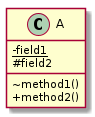
\includegraphics[width=3cm]{class-example.png}
  \centering
  \caption{diagramma delle classi realizzato con PlantUML}
\end{figure}
\begin{description}
  \item [Nomi e visibilità]: i nomi di classi, campi dati e metodi andranno indicati in minuscolo e scritti in lingua inglese.
        Inoltre, come in un vero e proprio linguaggio di programmazione, in UML è possibile indicare la visibilità di una variabile o di un metodo:
        \begin{description}
          \item [-]: visibilità privata
          \item [\#]: visibilità protetta
          \item [+]: visibilità pubblica
          \item [\textasciitilde]: visibilità a livello di package
        \end{description}
  \item[Altre convenzioni]:
        \begin{itemize}
          \item I campi dati e i metodi statici devono essere sottolineati.
          \item Utilizzare \textit{{abstract}} per indicare classi astratte.
          \item Fare uso di \textit{<<interface>>} per indicare interfacce.
          \item Il tipo delle variabili e il tipo di ritorno va posto dopo il nome della variabile o del metodo in questione. Ad esempio:
                \begin{center}
                  \textit{-field1: String} \\\textit{+method1: int}
                \end{center}
        \end{itemize}
  \item [Relazioni]: una relazione di dipendenza indica una dipendenza logica presente tra due elementi del diagramma e si ha quando la modifica di un oggetto implica il cambiamento di un altro oggetto.
        Esistono molteplici tipi di dipendenze e ognuna induce differenti gradi di dipendenza tra gli oggetti.
        Compito del progettista sarà quello di minimizzare il numero di dipendenze, utilizzandole solo ove necessario al fine di attribuire un valore aggiunto al significato del proprio diagramma.
        Di seguito verranno elencate i tipi di relazioni di dipendenza possibili, ordinati per grado di dipendenza crescente.
        \begin{description}
          \item [Dipendenza]: la dipendenza può verificarsi in due casi:
                \begin{itemize}
                  \item Una classe A ha un metodo che riceve in input un'istanza di B.
                  \item Una classe A crea un oggetto di tipo B.
                \end{itemize}
                Inoltre, per indicare il tipo di dipendenza useremo principalmente due parole chiave:
                \begin{description}
                  \item [\textit{<<call>>}]: A invoca operazioni di B.
                  \item [\textit{<<create}]: A crea istanze di B.
                \end{description}
                La dipendenza si indica con una freccia tratteggiata come illustrato nell'immagine sottostante.
                \begin{figure}[H]%
                  \label{fig:dipendenza}
                  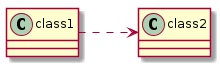
\includegraphics[width=5cm]{dipendenza.png}
                  \centering
                  \caption{Esempio di relazione di dipendenza}
                \end{figure}
          \item [Associazione]: l'associazione si verifica quando un oggetto di classe A ha un campo dati di tipo B.
                L'associazione si indica con una linea continua come nell'immagine sottostante:
                \begin{figure}[H]%
                  \label{fig:associazione}
                  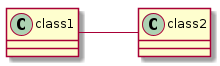
\includegraphics[width=5cm]{associazione.png}
                  \centering
                  \caption{Esempio di relazione di associazione}
                \end{figure}
          \item [Aggregazione]: l'aggregazione prevede che una classe di tipo A crei esplicitamente tramite il proprio costruttore degli oggetti di tipo B.
                L'aggregazione si rappresenta tramite una linea continua e un diamante che sta graficamente dalla parte di chi crea la dipendenza. Ad esempio:
                \begin{figure}[H]%
                  \label{fig:aggregazione}
                  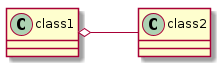
\includegraphics[width=5cm]{aggregazione.png}
                  \centering
                  \caption{Esempio di relazione di aggregazione}
                \end{figure}
          \item [Composizione]: la composizione è una forma di aggregazione più forte e si ha quando un oggetto di classe A gestisce completamente gli oggetti di tipo B.
                La composizione si rappresenta allo stesso modo dell'aggregazione, ma a differenza di quest`ultima il diamante è colorato di nero.
                \begin{figure}[H]%
                  \label{fig:composizione}
                  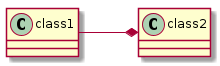
\includegraphics[width=5cm]{composizione.png}
                  \centering
                  \caption{Esempio di relazione di composizione}
                \end{figure}
          \item [Ereditarietà]: l'ereditarietà si ha quando un classe B deriva da una classe di tipo A.
                Ovviamente è preferibile ereditare da classi astratte o interfacce, mentre l'ereditarietà da tipi concreti sarebbe in ogni caso da evitare. Si rappresenta così:
                \begin{figure}[H]%
                  \label{fig:ereditarieta}
                  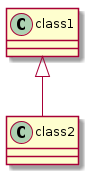
\includegraphics[width=2.1cm]{ereditarieta.png}
                  \centering
                  \caption{Esempio di relazione di ereditarietà}
                \end{figure}
        \end{description}
  \item [Molteplicità]: la molteplicità è uno strumento che permette di specificare quanti oggetti posso fare parte dell'associazione.
        Ogni molteplicità è una sigla costituita da numeri e simboli.
        Elenchiamo quelle di cui i progettisti dovranno fare uso:
        \begin{description}
          \item [1]: una classe A ha una e una sola istanza di classe di B associata.
          \item [0..1]: una classe A può avere zero o una istanze di classe B associata.
          \item [0..*]: una classe A può avere zero o più istanza di classe B associata.
          \item [*]: una classe A deve avere più istanze di B associate.
        \end{description}
\end{description}

\subparagraph{Diagrammi di package}%
\label{subp:diagrammi_di_package}
I diagrammi di package sono utili per rappresentare elementi appartenenti ad uno stesso namespace.
Hanno un'etichetta che identifica il nome, il quale deve essere in minuscolo e in inglese e possono contenere al loro interno altri package o classi.
Inoltre le dipendenze tra package si indicano con frecce tratteggiate e dovrebbero tutte seguire la medesima direzione.
\begin{figure}[H]%
  \label{fig:package}
  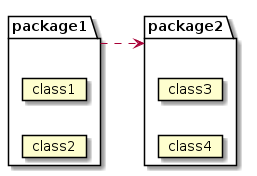
\includegraphics[width=5cm]{package.png}
  \centering
  \caption{diagramma dei package realizzato con PlantUML}
\end{figure}

\subparagraph{Diagrammi delle attività}%
\label{diagrammi_delle_attivita}%
I diagrammi delle attività rappresentano l'insieme delle azioni che ne costituiscono il funzionamento. Un tipico diagramma delle attività in PlantUML è:
\begin{figure}[H]%
  \label{fig:attività}
  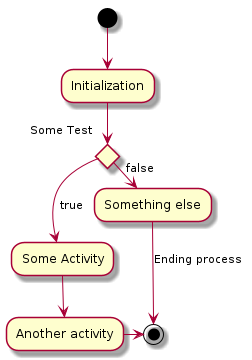
\includegraphics[width=5cm]{attivita.png}
  \centering
  \caption{diagramma delle attività realizzato con PlantUML}
\end{figure}
Gli elementi essenziali che li compongono sono:
\begin{itemize}
  \item Nodo iniziale
  \item Nodo finale
  \item Nodi di Branching
  \item Nodi di merge
  \item Fork e join.
\end{itemize}
I diagrammi di attività si basano sulla produzione e consumo di token.
Ogniqualvolta inizia il flusso di esecuzione e quindi ci trova nel nodo iniziale si genera un token.
Branching e merging consumano e producono un token, la fork produce un token per ogni processo in parallelo in esecuzione mentre la join li consuma tutti e ne genera uno.
Infine il nodo finale consuma tutti i token.
Altri elementi che possono essere utilizzati per realizzare diagrammi di attività più precisi sono:
\begin{itemize}
  \item Swimlanes
  \item Segnali
\end{itemize}
\begin{description}
  \item[Nodo iniziale]: il nodo iniziale è presente in ogni diagramma e delinea il punto di inizio di ogni diagramma delle attività. In PlantUML lo si rappresenta mediante un cerchio colorato di nero come nella figura:
        \begin{figure}[H]%
          \label{fig:nodo_iniziale}
          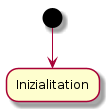
\includegraphics[width=3cm]{nodo-iniziale.png}
          \centering
          \caption{Esempio di nodo iniziale}
        \end{figure}
  \item[Nodo finale]: il nodo finale è presente in ogni diagramma e rappresenta il termine del flusso di esecuzione.
        In plantuml lo si raffigura come un cerchio contenente un altro cerchio colorato di nero:
        \begin{figure}[H]%
          \label{fig:nodo_finale}
          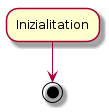
\includegraphics[width=3cm]{nodo-finale.png}
          \centering
          \caption{Esempio di nodo finale}
        \end{figure}
  \item[Nodi di branching]: i nodi di branching modellano delle decisioni.
        Hanno una guardia che indica quale test deve essere soddisfatto che si indica tramite un etichetta da affiancare al nodo di branching.
        Tali nodi si raffigurano mediante rombi vuoti e generalmente distinguono due branch:
        \begin{figure}[H]%
          \label{fig:nodo_di_branch}
          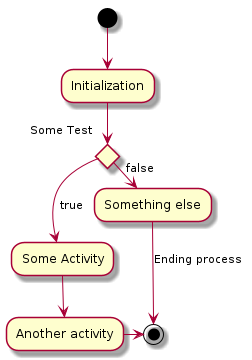
\includegraphics[width=5cm]{nodo-di-branch.png}
          \centering
          \caption{Esempio nodo di branching}
        \end{figure}
  \item[Nodi di merge]: i nodi di merge sono il punto in cui i rami generati da un nodo di branching tornano ad unirsi.
        Hanno la stessa rappresentazione dei nodi di branching.
        \begin{figure}[H]%
          \label{fig:nodo_di_merge}
          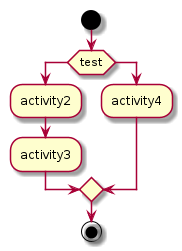
\includegraphics[width=5cm]{nodo-di-merge.png}
          \centering
          \caption{Esempio di nodo di merge}
        \end{figure}
  \item[Fork e join]: Fork e join sono necessari a rappresentare l'esecuzione parallela e concorrente.
        Ogniqualvolta il flusso di esecuzione incontra una fork il flusso di esecuzione diventa pari al numero di frecce uscenti dalla fork.
        Non è possibile terminare il flusso con più linee di esecuzione contemporaneamente attive ma è necessario che ci sia successivamente una join che ripristini l'unico flusso iniziale.
        Fork e join si rappresentano allo stesso modo, tramite una barra orizzontale colorata di nero. Ad esempio:
        \begin{figure}[H]%
          \label{fig:fork_e_join}
          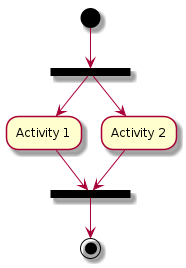
\includegraphics[width=5cm]{fork-e-join.png}
          \centering
          \caption{Esempio di fork e join}
        \end{figure}
  \item[Swimlanes]: Le Swimlanes sono strutture da poco introdotte in PlantUML che rendono esplicito di chi è la responsabilità nell'esecuzione. Si rappresentano così:
        \begin{figure}[H]%
          \label{fig:swimlanes}
          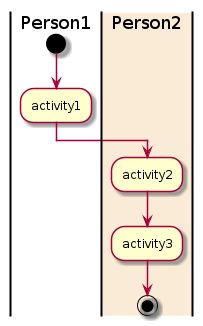
\includegraphics[width=5cm]{swimlanes.png}
          \centering
          \caption{Esempio di swimlanes}
        \end{figure}
  \item[Segnali]: I segnali servono per gestire eventi.
        PlantUML non offre un buon supporto per i segnali e ne offre una versione in beta.
        Ne esistono di due tipi:
        \begin{itemize}
          \item Segnali di input
          \item Segnali di output.
        \end{itemize}
  \item [Input]: i segnali di input aspettano una risposta proveniente dall'esterno.
        Possono essere la prima azione del diagramma.
        Si rappresentano così:
        \begin{figure}[H]%
          \label{fig:input}
          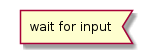
\includegraphics[width=5cm]{input.png}
          \centering
          \caption{Esempio segnale di input}
        \end{figure}
  \item [Output]: i segnali di output chiedono che venga inserito un input dall'esterno.
        Inoltre non possono essere la prima azione del diagramma.
        La loro rappresentazione è la seguente:
        \begin{figure}[H]%
          \label{fig:segnale_di_output}
          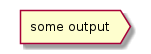
\includegraphics[width=5cm]{output.png}
          \centering
          \caption{Esempio segnale di output}
        \end{figure}
\end{description}

\subparagraph{Diagrammi di sequenza}%
\label{subp:diagrammi_di_sequenza}
I diagrammi di sequenza rappresentano dettagliatamente come gli oggetti interagiscono tra di loro mediante messaggi.
Ogni entità del diagramma è collegata mediante una linea tratteggiata verticale ad un'altra entità con lo stesso contenuto.
Tale linea indica il passare del tempo.
Le entità del diagramma si scambiano messaggi sotto forma di frecce che assumono una diversa struttura a seconda del tipo di messaggio che si sta inviando.
Segue un elenco delle tipologie di messaggi che due entità possono scambiarsi:
\begin{description}
  \item [Messaggio sincrono]: corrisponde alla chiamata di un metodo dal quale si attende un valore di ritorno.
        Lo si indica con una freccia continua nera piena accompagnata da un'etichetta contenente il tipo di metodo chiamato nella forma \textit{nomeMetodo (listaParametri)} dove la firma del metodo deve essere in lingua inglese e la lista di parametri deve essere nella forma \textit{nomeParametro1:tipo1, nomeParametro2:tipo2,\ldots}.
  \item [Messaggio asincrono]: corrisponde alla chiamata di un metodo dal quale non si attende nulla.
        Lo si indica con una freccia nera non piena accompagnata da un'etichetta identica a quella utilizzata per messaggi sincroni.
  \item [Messaggio di ritorno]: corrisponde ad un messaggio contenente il valore ritornato dalla chiamata di un metodo.
        Lo si indica con una freccia tratteggiata nera non piena accompagnata da un'etichetta contenente il tipo di valore ritornato.
  \item [Messaggio di creazione]: rappresenta un messaggio che chiede la creazione di un nuovo oggetto.
        Lo si indica con una freccia tratteggiata non piena seguita da un rettangolo contenente l'oggetto creato e accompagnata da un'etichetta contenente la parola \textit{<<create>>}.
  \item [Messaggio di distruzione]: rappresenta un messaggio che chiede la distruzione di un oggetto.
        Lo si indica con con una linea nera  seguita da una X e accompagnata da un'etichetta contenente la parola \textit{<<destroy>>}.
\end{description}
Un esempio di diagramma di sequenza corretto realizzato con PlantUML è il seguente:
\begin{figure}[H]%
  \label{fig:sequenza}
  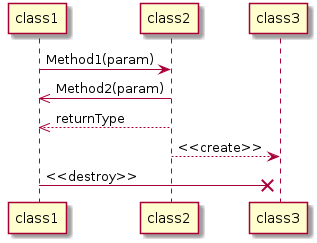
\includegraphics[width=7cm]{sequenza.png}
  \centering
  \caption{diagramma di sequenza realizzato con PlantUML}
\end{figure}
È possibile inoltre utilizzare delle cosiddette barre di attivazione per rendere immediatamente visibile a chi osserva il diagramma quando un'entità è attiva.
L`uso delle barre di attivazione non è obbligatorio ma è fortemente consigliato.
Il diagramma di prima con le barre di attivazione apparirebbe così:
\begin{figure}[H]%
  \label{fig:barre_attivazione}
  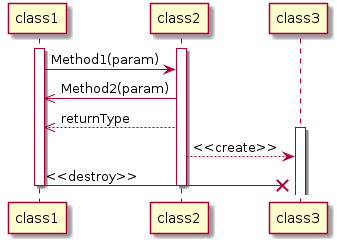
\includegraphics[width=7cm]{barre-attivazione.png}
  \centering
  \caption{Esempio barre di attivazione}
\end{figure}
Per modellare in maniera approfondita le interazioni fra oggetti è consigliato ai progettisti l'uso dei frame d'interazione introdotti in UML 2.
Tali frame si rappresentano come dei rettangoli a cui viene associata un'etichetta che indica il tipo di frame d'interazione.
Un esempio di diagramma di sequenza con i frame d'interazione è il seguente:
\begin{figure}[H]%
  \label{fig:frame_di_interazione}
  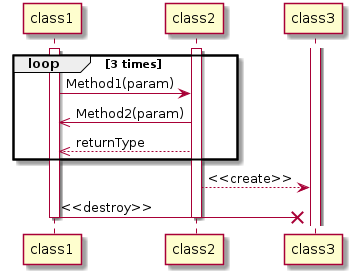
\includegraphics[width=7cm]{frame-interazione.png}
  \centering
  \caption{Esempio frame di interazione}
\end{figure}
Esistono diverse etichette per identificare i frame d'interazione. I progettisti dovranno attenersi alle seguenti:
\begin{description}
  \item [Alt]: indica frammenti alternativi che verranno eseguiti solo se la guardia è verificata.
  \item [Opt]: indica un frammento che viene eseguito solo se la condizione specificata è verificata.
  \item [Par]: indica frammenti da eseguire in parallelo.
  \item [Loop]: indica che il frammento può essere eseguito più volte, la base dell'iterazione è indicata dalla guardia.
  \item [Region]: indica una sezione critica. Il frammento può essere eseguito da un solo thread.
  \item [Neg]: indica un'interazione non valida.
  \item [Ref]: si riferisce ad un'interazione definita in una diagramma.
  \item [Ad]: si utilizza per racchiudere un intero diagramma di sequenza.
\end{description}

\paragraph{Codifica}%
\label{par:codifica}
L'attività di codifica consiste nell'implementazione delle specifiche del prodotto definite nelle attività precedenti.
Questa sezione ha lo scopo di evitare qualsiasi tipo di inconsistenza e rendere il codice più omogeneo possibile.
Questa attività viene svolta dal ruolo del programmatore, in quanto dispone delle conoscenze tecniche per eseguire le scelte effettuate nell'attività di progettazione e quindi sviluppare il prodotto di Stalker.

\subparagraph{Nomi dei file e delle variabili}%
\label{subp:nomi_file_e_variabili}
I nomi dei file:
\begin{itemize}
  \item Devono essere univoci e significativi.
  \item Devono rispettare le condizioni del linguaggio che contengono, se presenti.
\end{itemize}
I nomi delle variabili:
\begin{itemize}
  \item Devono essere chiari, descrittivi e possibilmente brevi.
  \item Devono essere significativi, relativi al contesto e alla loro utilità.
  \item Non devono somigliare tra loro, per evitare confusione a chi scrive il codice e a chi lo legge.
  \item Devono rispettare le condizioni del linguaggio in cui vengono usate, se presenti.
  \item Devono essere necessariamente scritti in lingua inglese.
\end{itemize}

\subparagraph{Commenti}%
\label{subp:commenti}
Il programmatore è tenuto ad inserire commenti dove ritiene che questo possa migliorare la leggibilità del codice.
In questo caso, i commenti devono essere chiari e nello stesso tempo sintetici, per non distrarre dal contesto.
Per contro, i commenti vanno omessi dove il codice è auto-esplicativo.

\subparagraph{Complessità ciclomatica}%
\label{subp:complessita_ciclomatica}
Va evitato il più possibile l’annidamento di più strutture di controllo.
Una buona prassi da rispettare è non andare oltre i tre livelli di annidamento, in quanto semplifica la leggibilità e il tempo di debugging.

\subparagraph{Ereditarietà}%
\label{subp:ereditarieta}
Una cattiva prassi è utilizzare l’ereditarietà tra classi concrete, ovvero che hanno stato, a causa del riuso del codice e dei problemi ``a cascata'' che si possono generare da una classe base alle sue classi derivate.
L'ottima prassi da applicare è utilizzare l'ereditarietà di interfacce, in modo da riutilizzare il comportamento dei metodi astratti definiti nelle interfacce.
Ergo, è da preferire la composizione sopra l'ereditarietà, adottando il principio di “Composition over inheritance”.

\subparagraph{Indentazione}%
\label{subp:indentazione}
Le indentazioni devono rispettare le seguenti specifiche:
\begin{itemize}
  \item I blocchi annidati devono essere indentati con quattro (4) spazi
  \item Non è possibile utilizzare tabulazioni per l'indentatura, è obbligatorio utilizzare il numero di spazi appropriato
  \item Tutto il codice facente parte di un blocco deve essere indentato a livello di quel blocco.
\end{itemize}

\subparagraph{Parentesizzazione}%
\label{subp:parentesizzazione}
La parentesizzazione deve rispettare le seguenti norme:
\begin{itemize}
  \item I blocchi di codice devono essere necessariamente racchiusi tra parentesi graffe
  \item Le parentesi graffe iniziano sempre nella stessa riga del codice che le precede.
\end{itemize}
% subp:parentesizzazione (end)

\subparagraph{Lunghezza dei metodi}%
\label{subp:lunghezza_metodi}
Quando possibile è auspicabile limitare la lunghezza dei metodi per circoscrivere lo scopo del metodo e aumentarne la leggibilità.
% subp:lunghezza_metodi (end)

\subparagraph{TODO}%
\label{subp:TODO}
Gli sviluppatori sono invitati a usare il commento ``TODO'' per il codice temporaneo e per il codice ancora da implementare così da facilitare la comprensione del compito ancora da svolgere.
Se i ``TODO'' hanno una data di scadenza essa va indicata nel commento.
% subp:TODO (end)

\subparagraph{Inizializzazione variabili}%
\label{subp:inizializzazione_variabili}
Le varabili andrebbero inizializzate il prima possibile: ad ogni definizione andrebbe affiancata l'inizializzazione della variabile, se ciò non è possibile va fatto quanto prima.
% subp:inizializzazione_variabili (end)

\subparagraph{Ricorsione}%
\label{subp:ricorsione}
La ricorsione come paradigma di programmazione va usata con moderazione poiché un uso sconsiderato può portare a una maggiore occupazione di memoria rispetto alla controparte iterativa.
L'uso della ricorsione andrebbe motivato con appositi commenti.
% subp:ricorsione (end)
% subp:indentazione (end)
\subsubsection{Strumenti}%
\label{subs:strumenti}

\paragraph{PlantUML}%
\label{par:plantuml}
Per la costruzione dei diagrammi UML il team ha deciso di utilizzare \glossario{PlantUML}\@.
È un software open source che permette la costruzione di diagrammi UML a partire dalla scrittura di codice in un linguaggio di markup dedicato. GruppOne ha valutato positivamente tale strumento in quanto:

\begin{itemize}
  \item Gli aspetti grafici di costruzione dei diagrammi sono demandati al software sottostante.
  \item La sua natura testuale e dichiarativa permette di attuare un versionamento efficace dei diagrammi attraverso strumenti che già utilizziamo.
  \item Permette di scrivere agevolmente i diagrammi dei casi d'uso, delle classi, di sequenza e di package.
\end{itemize}

In seguito a difficoltà nell'utilizzo del package apposito di \LaTeX{}, abbiamo deciso di pre-compilare separatamente i diagrammi utilizzando le funzionalità esposte dalla \glossario{Command Line Interface} di PlantUML\@.

Posizionarsi nella cartella contenente la documentazione di progetto ed eseguire il comando:

\begin{minted}{bash}
  java \
    -jar \
    $PLANTUML_JAR \
    -checkmetadata \
    -charset UTF-8 \
    -x **/commons/style/*.pu \
    -o img \
    **/**.pu
\end{minted}

La corretta esecuzione del comando richiede di aver impostato la variabile d'ambiente \verb|PLANTUML_JAR| al percorso completo del file \verb|plantuml.jar| reperito dal sito del progetto.

In questo modo vengono generate le immagini che sono effettivamente incluse nei documenti dal comando dato in~\ref{par:LaTeX}.

\subparagraph{Esempio diagramma PlantUML}%
\label{subp:esempio_diagramma_plantuml}

\begin{minted}{text}
  @startuml
  left to right direction
  skinparam packageStyle rectangle
  actor customer
  actor clerk
  rectangle checkout {
    customer -- (checkout)
    (checkout) .> (payment) : include
    (help) .> (checkout) : extends
    (checkout) -- clerk
  }
  @enduml
\end{minted}

Il risultato grafico del codice è presentato in~\ref{fig:esempio_caso_duso}

\begin{figure}[H]%
  \label{fig:esempio_caso_duso}
  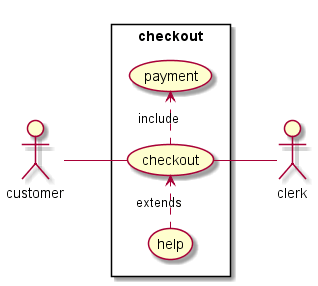
\includegraphics[width=8cm]{use-case-example.png}
  \centering
  \caption{diagramma dei casi d'uso realizzato con PlantUML}
\end{figure}

% subp:esempio_diagramma_plantuml (end)

\paragraph{Package pgfgantt}%
\label{par:pgfgantt}

Per i diagrammi di Gantt il gruppo ha scelto di utilizzare pgfgantt, un package disponibile per \LaTeX{} che sfrutta il linguaggio \glossario{PGF} e il rispettivo omonimo interprete.
PGF è in grado di produrre rappresentazioni grafiche vettoriali, e pgfgantt fornisce dei comandi \TeX{} che fungono da astrazioni per le direttive di basso livello.
Un diagramma di Gantt viene quindi costruito attraverso uno o più comandi di titolo, seguiti da una combinazione di comandi specifici per inserire gruppi, ``barre'' (cioè attività) o milestone, oppure per collegare due elementi.

L'integrazione dei diagrammi nel documento avviene durante la compilazione del documento effettuata attraverso il comando dato in~\ref{par:LaTeX}.

% par:pgfgantt (end)

\subsubsection{Metriche di processo}%
\label{subs:sviluppo/metriche_di_processo}

\paragraph{MPS-ROS: Requisiti obbligatori soddisfatti}% in questo caso NON ci va il "\@". chktex 13
\label{par:MPS-ROS_requisiti_obbligatori_soddisfatti}

La metrica requisiti obbligatori soddisfatti indica la percentuale di requisiti obbligatori soddisfatti sul numero totale di requisiti obbligatori. La formula è la seguente:
\[
  \frac{requisiti\ obbligatori\ soddisfatti}{requisiti\ obbligatori\ totali}\cdot 100
\]

\paragraph{MPS-NFV: Nomi di file e variabili non normati}% in questo caso NON ci va il "\@". chktex 13
\label{par:MPS-NFV_nomi_file_variabili_non_normati}

I nomi dei file o delle variabili devono seguire delle specifiche regole per essere più chiare possibile.

\textbf{Metrica:} numero di nomi di variabili o di titoli di metodi o classi che non rispettano le norme stabilite.

\paragraph{MPS-CNN: Commenti non normati}% in questo caso NON ci va il "\@". chktex 13
\label{par:MPS-CNN_commenti_non_normati}

I commenti devono essere scritti seguendo le norme indicate per essere comprensibili.

\textbf{Metrica:} numero di commenti che non rispettano le norme indicate.

\paragraph{MPS-CCE: Complessità ciclomatica eccessiva}% in questo caso NON ci va il "\@". chktex 13
\label{par:MPS-CCE_complessita_ciclomatica_eccessiva}
una sezione di codice è il numero di cammini linearmente indipendenti attraverso il codice sorgente

Il grado di difficoltà di testare un metodo è proporzionale al numero di cammini linearmente indipendenti: più è alto il numero di cammini, più è alto il grado di complessità.
Ne deriva inoltre un'esecuzione più lenta del metodo. E' quindi buona norma limitare il numero massimo di cammini.
La formula che calcola la complessità ciclomatica è la seguente:
\[
  v(G) = e - n + p
\]
dove:
\begin{description}
  \item[v(G):] complessità ciclomatica del grafo G. % chktex 36
  \item[e:] numero di archi del grafo.
  \item[n:] numero di nodi del grafo.
  \item[p:] numero di componenti connesse.
\end{description}
\textbf{Metrica:} numero di metodi che hanno \[v(G) > 3.\]

\paragraph{MPS-ICC: Classi che implementano classi concrete}% in questo caso NON ci va il "\@". chktex 13
\label{par:MPS-ICC_classi_implementano_concrete}
L'ereditarietà tra classi andrebbe evitata poiché la presenza di dipendenze tra più componenti ne ostacola la modifica e la verifica.

\textbf{Metrica:} numero di classi che ereditano un'altra classe concreta.

% par:MPS-014_classi_implementano_concrete (end)


\end{document}
